\documentclass{mcmthesis}
\mcmsetup{CTeX = false,   % 使用 CTeX 套装时,设置为 true
        tcn =2008722, problem = C,
        sheet = true, titleinsheet = true, keywordsinsheet = true,
        titlepage = false, abstract = true}
\usepackage{newtxtext}%\usepackage{palatino}
\usepackage{url}
\usepackage{geometry}
\geometry{left=1.3in,right=1.3in,bottom=1.25in}
\usepackage{chngpage}
\usepackage{array}
\usepackage{booktabs}
\usepackage{threeparttable}
\usepackage{longtable}
\newcommand{\upcite}[1]{\textsuperscript{\textsuperscript{\cite{#1}}}}
\usepackage[numbers,sort&compress]{natbib}
%%% 实现参考文献标号在右上角
\usepackage{lipsum}
\title{Thousands of Things We can Learn from the Data}
\usepackage{verbatim}
%\usepackage{epstopdf}
%\usepackage{float}
%\usepackage{subfig}
%\usepackage{amsmath}
%\usepackage{cases}
\begin{document}
\begin{abstract}

This is the age of information explosion. Numbers, text, video, and audio are all information. How to extract the instructive information we are interested in from the large amount of data is crucial. In this article, our team built an evaluative model based on user reviews.

From the basic information about the data, we find that the number of comments is increasing exponentially, and more and more consumers choose to shop online, among which beauty and baby products are more popular among consumers. To understand consumer preferences, word frequency statistics and sentiment analysis of product reviews were performed using TextBlob, a Natural Language Processing library in Python. It is found from the word cloud that consumers are most concerned about the quality and price of products. Specific quality descriptor of text-based reviews--"love" strongly is associated with rating levels.

In order to understand the product reputation and predict whether the product will be successfully promoted , through the scoring model based on user reviews , we define the product reputation score and product future development scores , and we can understand the status of different products ' reputation and whether the product will be successful in the future . In order to understand whether the product evaluation content has a " group effect " , We use the moving average algorithm in the time series to perform a typical correlation analysis between the predicted data and the original data onto the product of a large number of reviews. We found that customers are more likely to write some types of review after seeing a series of low star ratings.

Our model is powerful because it is extensible and easy to understand. One of the weaknesses for this model is that it is too subjective without strong logic. Finally, we performed sensitivity analysis and extended the model.
\begin{keywords}
TF-IDF, \ NLP, \ Canonical Correlation Analysis
\end{keywords}
\end{abstract}
\maketitle
%% Generate the Table of Contents, if it's needed.
\thispagestyle{empty}
\tableofcontents

%\newpage
%\thispagestyle{empty}
%\title{fish of scotland}
%\lipsum{5}

%%
%Generate the Memorandum, if it's needed.
\newpage
\memoto{Marketing Director of Sunshine Company}
\memofrom{MCM Team 2008722}
%\memosubject{}
\memodate{\today}

\begin{memo}[Letter]
	Dear Sir:
	
	We are your consultants and we are honored to help you analyze your company's three new product online sales strategies.After a period of hard work, we have achieved good results and have completed the questions and requirements raised by your company. This letter is to report to you our latest findings and results. We identified key information from historical ratings and reviews provided by your company, and built an evaluation model based on user reviews, used it to describe online sales strategies, and identified potentially important design features to enhance product effectiveness. If you are interested, you can get a general understanding of our solution through my next elaboration. Of course, I will also do my best to convince you.
	
	First of all, thank you for your company's data center for the three historical data files that provided us with key data support for our research. Although the data file contains a small amount of abnormal data, we have used the Python programming language to perform data cleaning, which can ensure the validity of the data and avoid the interference caused by dirty data.
	
	Next, we performed quantitative or qualitative analysis on the more critical data in the data file, including star ratings, reviews, and help ratings, and discussed the internal and mutual relationships between them. We found that the number of online shoppers has grown exponentially after 2008, which indicates that online shopping is becoming more popular with customers. We have reason to believe that online sales will defeat traditional market sales, and online shopping will become a new habit for people in the new era. It is strongly recommended that Sunshine Company develop and focus on online sales.
	
	After the three products are launched, your company can use it to get the product score of the product based on rating and review data, and the product score can intuitively understand the product's benefits. Data that affect product scores include star ratings for reviews, total reviews, help ratings, purchase confirmations, vines, polarity and subjectivity of review content. Among them, polarity and subjectivity are the results of sentiment analysis on the content of comments using Python's TextBlob library. We build models based on these factors, and they are given corresponding weights to ensure that they can have a corresponding effect on the results.
	
	Fortunately, there is no problem with the date format of the data. We have built a time series model based on product reputation for analysis. The data that affects product reputation include star ratings for reviews, help ratings, purchase confirmation, vine, and polarity of review content. And subjectivity.  Because there are many gaps in the time of the data, that is, the time when the reviews occur is not continuous, we use Python's matplotlib library to draw a time series diagram of the discontinuity of the reputation of a certain product. Through analysis, we have established a measure of time to better demonstrate the change in the reputation of the product in the market. Vine reviewers have a greater impact on product reputation, so it is strongly recommended that your company invite vine reviewers to use the product and give reviews to improve reputation.
	
	To better predict the success and failure of potential products, we focus on analyzing those products with higher and lower scores, discuss some changes in star ratings and review content before success or failure, and define an indicator -Future development score. This indicator can indeed reflect product development potential.
	
	Before this research, we thought that most users would be more likely to write highly subjective reviews when they saw a series of high or low star ratings, but this is only a guess, after all, so we need to build math The model is validated. We analyzed the first ten reviews of eligible reviews and discussed the relationship between their star rating and the content and number of reviews. We have used a typical correlation analysis on them through the Spass software, and we believe that the content of the reviews does have a group effect. Therefore, in the initial stage of putting products on the online market, your company must pay attention to the initial reviews, which is very important for product development.
	
	Finally, because we need to find the relationship between specific quality descriptors and star ratings in review content, we used Python to perform word frequency statistics and sentiment analysis on the content of product reviews and obtained corresponding data. And analyzed by spass software, it was found that some special words have a strong correlation with star rating.
	
	Please believe that my solution will be helpful for your company's online sales strategy. If you still have some doubts, you may wish to take a look at our solutions, I believe we will definitely give you quality answers.
	You are welcome to contact us at any time for further cooperation.
	
	Sincerely,
	
	MCM \ Team 2008722 
	
\end{memo}

\newpage
\setcounter{page}{1}
%%

\section{Introduction}
\subsection{Background}

With the development of e-commerce and the improvement of the logistics service level, more and more people choose online shopping as a fast and convenient shopping method. With the development of big data and the massive increase of data, data plays an important role in business decision-making and company development. Customers can obtain information from other people's evaluations to decide whether to buy; companies can discover information from big data to better serve customers, increase efficiency, and enhance industry competitiveness.

\subsection{Restatement of the Problem}

For Sunshine's three online sales products to succeed, we first need to identify key patterns, relationships, metrics, and parameters that are relevant through reviews and ratings in the only available data given. Then our two major goals are 1. To clarify the sales strategy; 2. To discover the important characteristics that potentially affect sales and help improve product satisfaction. Finally, a series of requirements should be fully considered;

\begin{itemize}

\item Establish a data measurement mechanism: Once the hairdryer, microwave oven, and baby pacifier are sold online, the company can discover the product ’s customer preferences, sales, and areas worth improving based on market reactions (ratings, reviews).

\item Taking the time factor into consideration and establishing a time-based model, we can discuss the future development trends of each commodity, market competitiveness, and market reputation.

\item Combine text and rating metrics to predict whether a product will succeed in the market.


\item Consider whether a particular star rating will trigger similar comments from others.

\item Whether some special words are strongly related to ratings.

\end{itemize}

\subsection{Analysis of the Problem}

First, we need to perform sentiment analysis and word frequency extraction on the comments through Python's natural language processing library. Then build a model for data mining of text and data, including product reputation, keywords, comment validity, and product characteristics. Finally, give Sunshine some online sales strategies.

\newpage
\section{Assumptions}

\begin{itemize}

\item Suppose a user makes a review once they purchase a product, and the sales volume is considered to be equivalent to the number of reviews.

\item Assume that the product data set provided by Sunshine is in line with the laws of the online market, that is, no abnormal conditions have occurred in the period of the data set, such as the increase or decrease in product sales caused by natural disasters.

\item Suppose that the time interval between the user placing an order and receiving the goods in the data set is small, that is, the user comments shortly thereafter.

\item Treat orders with significant differences in ratings and reviews as normal orders.

\end{itemize}

\section{Notation}
\begin{table}[h]
\centering

\begin{tabular}{lll}
	\toprule
	Symbol\ quad\quad\quad\quad\quad\quad\quad\quad\quad &Significance  \\
	\midrule
	$ \mathbf{k}  $   &  Review Score
	\\
	$ \mathbf{s}  $   & Star Rating
	\\
	$ \mathbf{P}  $   & Polarity Score
	\\
	$ \mathbf{S}  $   & Subjective Score
	\\
	$  \mathbf{\beta_i} $   & Helpfulness Rating
	\\
	$\mathbf{r}   $   & Importance of Reviews
	\\
	$ (\boldsymbol{f1},\boldsymbol{f2},\boldsymbol{f3})  $   & Review Score, Product Score, Consumer True Evaluation Score
	\\
	$  \mathbf{p} $   &Each Reviewer's Credit for the Product's Reputation
	\\
	$ \psi_j $   &  Product j Potential Score
	\\
	$  \rho $   & Person Correlation Coefficient
	\\	
	$  Ras $     & Rating the average of stars
	\\
	$ \alpha $ & Significance level
	\\
	\bottomrule
\end{tabular}
\end{table}

\section{Model 1: Word Frequency Algorithm}

To determine the attribute information of each comment, we must first extract the valid information in the comment sentence. Then judge the words based on the extracted words. The TF-IDF algorithm is a statistical algorithm that can count the number of occurrences of a word in an article, and then find the frequency of the word. We use the frequency of words to characterize the importance of the word in the article.

Before performing word frequency statistics, we must also understand how computers extract words from articles. We know that extracting words is a very tedious task, and in the process, we have to consider multiple situations:

\begin{itemize}

\item Some simple words such as $'a', 'an', 'is', 'the' \cdots$ exist in large numbers and have no analytical significance, so when natural language processing is performed, such words are not considered, so stop Words are not considered.

\item For example, $'like'$, $'Like'$, and $likes$ have different capitalization and different word tenses. They should be regarded as one word, but they are treated as different words in this article for analysis.

\item When segmenting sentences with spaces and punctuation to extract words, some abbreviations such as $we'll$, $we're$, $pinkish-blue$ were difficult to separate, but they can be accurately performed in the NKTL library Division.

\end{itemize}

Python has many very powerful natural language toolkits that can save us a lot of time with seemingly simple but very complex operations. On the processing of stop words, we downloaded a stop word dataset \url{https://blog.csdn.net/shijiebei2009/article/details/39696523/}, which contains 891 words. When processing text data, we deleted $891 * 2 + 1$ words from the divided words, which took into account the capitalization of stopword words and unexplained space characters.

In the word frequency algorithm, the reason why we use the NLTK library to implement the TF-IDF algorithm is that the NLTK library can process multiple text contents into a combined calculation instead of only a single text.

\subsection{TF is Term Frequency}

TF indicates how often the keyword appears in the text. To prevent it from biasing towards longer text, this number is usually normalized. It is worth mentioning that for other considerations later, we also use the word frequency. The formula is as follows:

\begin{equation}
t f_{i j}=\frac{n_{i, j}}{\sum_{k}^t n_{k, j}}
\end{equation}

where\enspace\(n_{i, j}\) represents the number of times the i-th word appears in the file $d_j$;

t represents the number of all entries in the file $d_j$

The denominator is the sum of the number of occurrences of all terms in the file $d_j$.

\subsection{IDF is Inverse Document Frequency}

The main idea of TF-IDF is: if a word appears frequently in one article and rarely appears in other articles, it is considered that the word has good class discrimination ability and is suitable for classification. If fewer documents are containing the term t and the larger the IDF, it means that the term has good category discrimination ability\upcite{Baenagarc2012TF}. This is also in line with our goal of qualitative analysis of the evaluation content. The formula is as follows:

\begin{equation}
i d f_{i}=\log \frac{|D|}{\left|\left\{j: t_{i} \in d_{j}+1\right\}\right|}
\end{equation}

where\enspace\(|D|\) represents the number of texts studied;

$j: t_{i} \in d_ {j}$ represents the number of files containing the term ti. Adding 1 here is to avoid the situation where the denominator is 0.

\subsection{TF-IDF is Actually: TF * IDF}

The high word frequency in a particular file and the low file frequency of the word in the entire file set can generate a high weighted TF-IDF. Therefore, TF-IDF tends to filter out common words and retain important words. The formula is:

\begin{equation}
TF-I D F=T F * I D F
\end{equation}

\subsection{How to Track Sales Situation form This Modle}

By understanding the frequency of occurrences and comments, we can understand that consumers really care about the characteristics of the product, and we can analyze and obtain the places where consumers are not satisfied with the products and sales services. Sunshine can improve and strengthen these places.

\section{Model 2: Evaluation Model Based on User Reviews}

\subsection{Qualitative Analysis of Reviews}

Today's online shoppers have different definitions of good or bad products, but unless shoppers are particularly dissatisfied with a product, most of the time they will praise it. Because online product providers do not have the cost of appearance fees, etc., the products on the Internet are very cheap, and people tend to be more "sympathetic" to a cheaply purchased product. Frequently "OK, OK, OK" reviews like\upcite{zz}. The content of the review is the data that determines the true thinking of the buyer. We need to mine the true score of the product from the text data.

\begin{figure}[h]
\centering
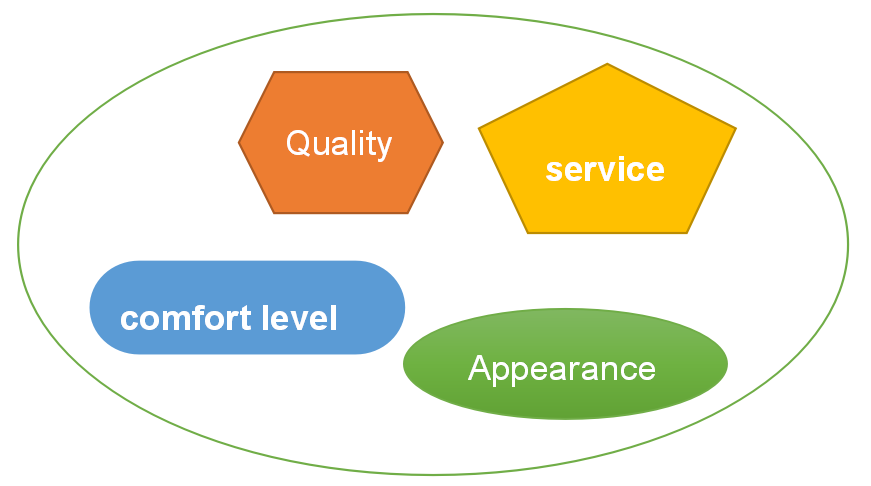
\includegraphics[width=6cm]{./figures/m1p.png}
\caption{The main content of the product review} \label{m1p}
\end{figure}

As can be seen in figure \ref{m1p}, the main content of the review includes four aspects: quality, service, comfort, and appearance. A large number of reviews also include subjective feelings after using the product. Therefore, it is necessary to carry out a sentiment analysis of goods.

TextBlob stands on the huge shoulders of NLTK and pattern, and both work well together, and can be used for in-depth research on general natural language processing (NLP) tasks such as part-of-speech tagging, noun phrase extraction, sentiment analysis, etc\upcite{Martinc2015Efficient}.
Affective and subjective classification: This is the area most studied in academia. It treats sentiment analysis as a text classification problem. Two sub-themes that have been studied extensively are:(1) classify documents with opinions as expressing positive or negative opinions, (2) classify sentences or clauses as subjective or objective, and subjective sentences or clauses as positive, negative or Neutral perspective. Sentiment analysis aims to find the author's overall sentiment in the reviewed text. For example, given a product review, it determines whether the reviewer's sentiment about the product is positive or negative. In this article, we used sentiment analysis to get two values: polarity, subjectivity. polarity indicates that the polarity score floats in the range [-1.0, 1.0]. The subjective score is floating in the range of [0.0, 1.0], where 0.0 is very objective and 1.0 is very subjective.

This article divides all comments into 5 categories for analysis:

1. Praise (pure praise, without any bad words about the product);

2. Praise (overall praise, with some dissatisfaction);

3. Middle evaluation (more objective evaluation, centered view);

4. Negative evaluation (due to some unexpected or service attitude, such as express delivery reasons);

5. Negative evaluation (due to the product itself, such as quality reasons).

Perform a qualitative analysis of the review content by polarity and get a review score:

\begin{equation}\label{m1gs1}
k_i=\left\{\begin{array}{lll}
1 & \text { bed review } & \text {if -1 $\leq$ polarity < 0 }\\
2 & \text { medium review } & \text {if polarity = 0 }\\
3 & \text { good review } & \text {if 0 < polarity $\leq$ 0 }
\end{array}\right.
\end{equation}

\begin{figure}[!htbp]
\centering
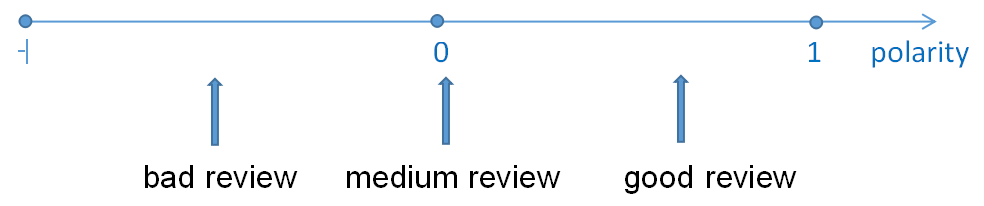
\includegraphics[width=8cm]{./figures/m11p.png}
\caption{Attribute analysis of comment content} \label{m11p}
\end{figure}

$k_i$ is the review score, which is based on consumer reviews. polarity indicates that the polarity score floats in the range [-1.0, 1.0]. The closer the polarity is to the product of the 1st name, the better the product is, and the closer the polarity is to the -1 of the name, the worse the product is. 0 means that the consumer's review of the product is neither a negative review nor a positive review, that is, a middle review, with a rating of 2.

\subsection{Importance of Reviews}

The importance of comments is reflected in four aspects:

\begin{itemize}

\item The larger the ratio of useful votes to the total votes, the greater the amount of information. Increase the importance by 1, but no more than 2;

\item If the customer ’s rating is high and the label is “green label”, the influence is greater and the importance is increased by 2;

\item If the customer's reviews are more objective, ie the subjectivity is smaller, the reviews are more important, and the importance is increased by 1;

\item If the customer did buy the product, the review has higher credibility and an increase of 1.

\end{itemize}

Based on the above description, get the importance of the comment:

\begin{equation}
r_{i}=\frac{\sum_{1}^{4}r_{ij}}{\mathbf{max} r_i}
\end{equation}

\begin{equation}
\beta_i=\left\{\begin{array}{ll}
\frac{helpful\quad votes}{total\quad votes} & \text { if total votes $\neq$ 0 } \\
0 & \text { else }
\end{array}\right.
\end{equation}

Among them:

$\beta_i$ is the ratio of useful votes;

$
r_{i1}=\left\{\begin{array}{ll}
2 & \text { if $\beta_i$ > 50\% } \\
1 & \text { if $\beta_i \leq $50\% } \\
0 & \text { $\beta_i$ = 0 }
\end{array}\right.
$
represents the importance attribute of the useful ticket;

$
r_{i2}=\left\{\begin{array}{ll}
2 & \text { if vine = Y } \\
0 & \text { else }
\end{array}\right.
$
represents the important attribute of the reviewer;

$
r_{i3}=\left\{\begin{array}{ll}
1 & \text { if $S_i$ <0.5  } \\
0 & \text { else }
\end{array}\right.
$
represents the objective degree attribute of the review;

$
r_{i4}=\left\{\begin{array}{ll}
1 & \text { if verified purchase = Y } \\
0 & \text { else }
\end{array}\right.
$
represents the objective degree attribute of the review;

\subsection{Output Model for Different Information}

\begin{equation}\label{q1}
f(\boldsymbol{k},\boldsymbol{r},\boldsymbol{s})=(\frac{1}{3}\boldsymbol{k}^T\cdot \boldsymbol{r},\eta \boldsymbol{s} + 5(1-\eta)\boldsymbol{r},\phi\boldsymbol{s} + \frac{5}{3}(1-\phi)\boldsymbol{k})=(\boldsymbol{f1},\boldsymbol{f2},\boldsymbol{f3})
\end{equation}
Where:

$f1_i$ represents the effective score of the review, ranging from $[0,1]$. This takes into account the review score obtained from the sentiment analysis of the text and the importance of the review. The effective score of reviews is to be able to filter out important reviews and is an important basis for providing customer opinions to Sunshine.

$f2_i$ represents the product score and ranges from $[0,5]$. Able to comprehensively reflect the value and quality of the product. This is essential for evaluating whether a product will succeed or fail. Because sometimes star ratings and reviews are contradictory, this is why we use a weighted method to coordinate the two. We know that reviews are entered manually, and it is impossible to violate the original evaluation of the consumer, and the star rating is clicked on the mouse, so it is likely to be wrong. A star rating of 1 or 2 appears, but reviews are good.

Why didn't we delete the data that star rating and review contradicted?

Because the data is given through the questions, we find that the data before 2008 are very small. If the original data is reduced, it is not good for data analysis.

$f3_i$ represents the true consumer evaluation score, ranging from $[0,5]$. This can reflect consumers' true feelings about buying products.

$\phi$ represents the weight of star ratings in consumers 'true evaluation scores, and $1- \phi$ represents the weight of review scores in consumers' true evaluation scores. In real consumer evaluation scores, we consider star ratings and evaluation scores to be equally important, so $\phi = 0.5$.

$\phi$ represents the weight of star rating in product score, and $1- \phi$ represents the weight of review score in product score. In product scores, evaluating effective scores is considered a more important factor than star ratings, so $\eta = 0.3$.

Once the three products are sold on the online market, Sunshine can measure and track product sales based on these three data. Sunshine Company can understand the pros and cons of the substantive factors such as product quality in the minds of consumers through product scores. It can also determine the true feelings of the product in the minds of consumers based on the true evaluation scores of consumers.

\section{ Results and Recommendations}
\subsection{Inform Online Sales Strategy}
First, we do some basic analysis of the known raw data to understand the basic situation of online sales. Then we raised a series of questions that the sun company might be interested in.

1. Is online shopping becoming more common in America?

2. Will online sales replace traditional marketing?

3. Whose user experience is better online than traditional sales?

4. What products are suitable for online sales?

\begin{figure}[h]
	\center
	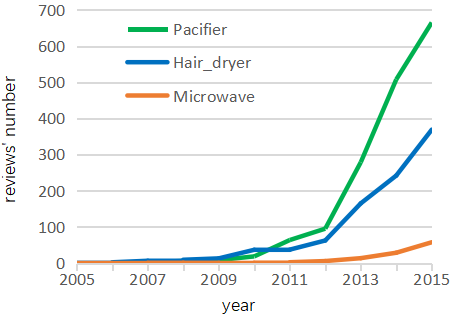
\includegraphics[width=6cm]{./figures/q1p1.png}
	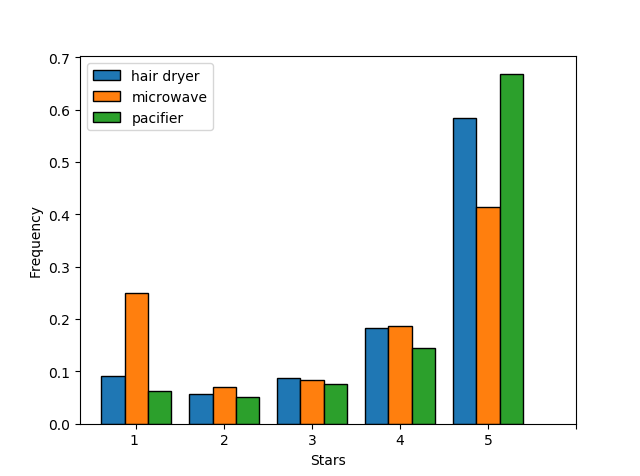
\includegraphics[width=6cm]{./figures/z1.png}
	\caption{Basic information description comparison chart} \label{z1_q1p1}
\end{figure}

We know that the number of comments is directly proportional to the number of online shoppers, so we can see the figure on the right as the relationship between the number of online shoppers and time. From the left chart, we can find that before 2008, very few people chose to shop online. After 2008, online shopping became more and more popular. To analyze the reasons, the subprime mortgage crisis in the United States in 2008 triggered the global financial crisis, which led to the failure of many banks and the collapse of small and medium-sized enterprises. In order to survive, many small businesses have switched to online sales, because it is known that online sales cost is small, with no rent, sales staff.

We found that the number of online shoppers increased exponentially after 2008, indicating that online shopping is becoming more and more popular with customers. We have reasons to believe that online sales will beat traditional marketing, and online shopping will become the new shopping habit of people in the new era. Here we strongly suggest the sun company to develop an online sales business.

Pacifiers are baby products, hairdryers are beauty products, and microwave ovens are large appliances. On the left, we found that compared to hairdryers and pacifiers, the number of microwave reviews is very small, that is, the number of people who buy microwave ovens online is very small. Combined with the picture on the right, the one-star microwave oven can be found to be very large, which indicates that consumers do not like to buy large appliances online. In summary, beauty and baby products are more suitable for online sales.

The figure on the right shows the star distribution map of online reviews of three kinds of products. The frequency of five-star pacifiers and hairdryer is more than 50\%, which indicates that most people have a good online shopping experience for these products. Everyone can buy things that are both cheap and easy to use to meet their needs.

Through the NLTK of Python, the TF-IDF algorithm is used to calculate the word frequency of comments, and the word cloud graph is drawn as follows through a word cloud.

\begin{figure}[h]
	\centering
	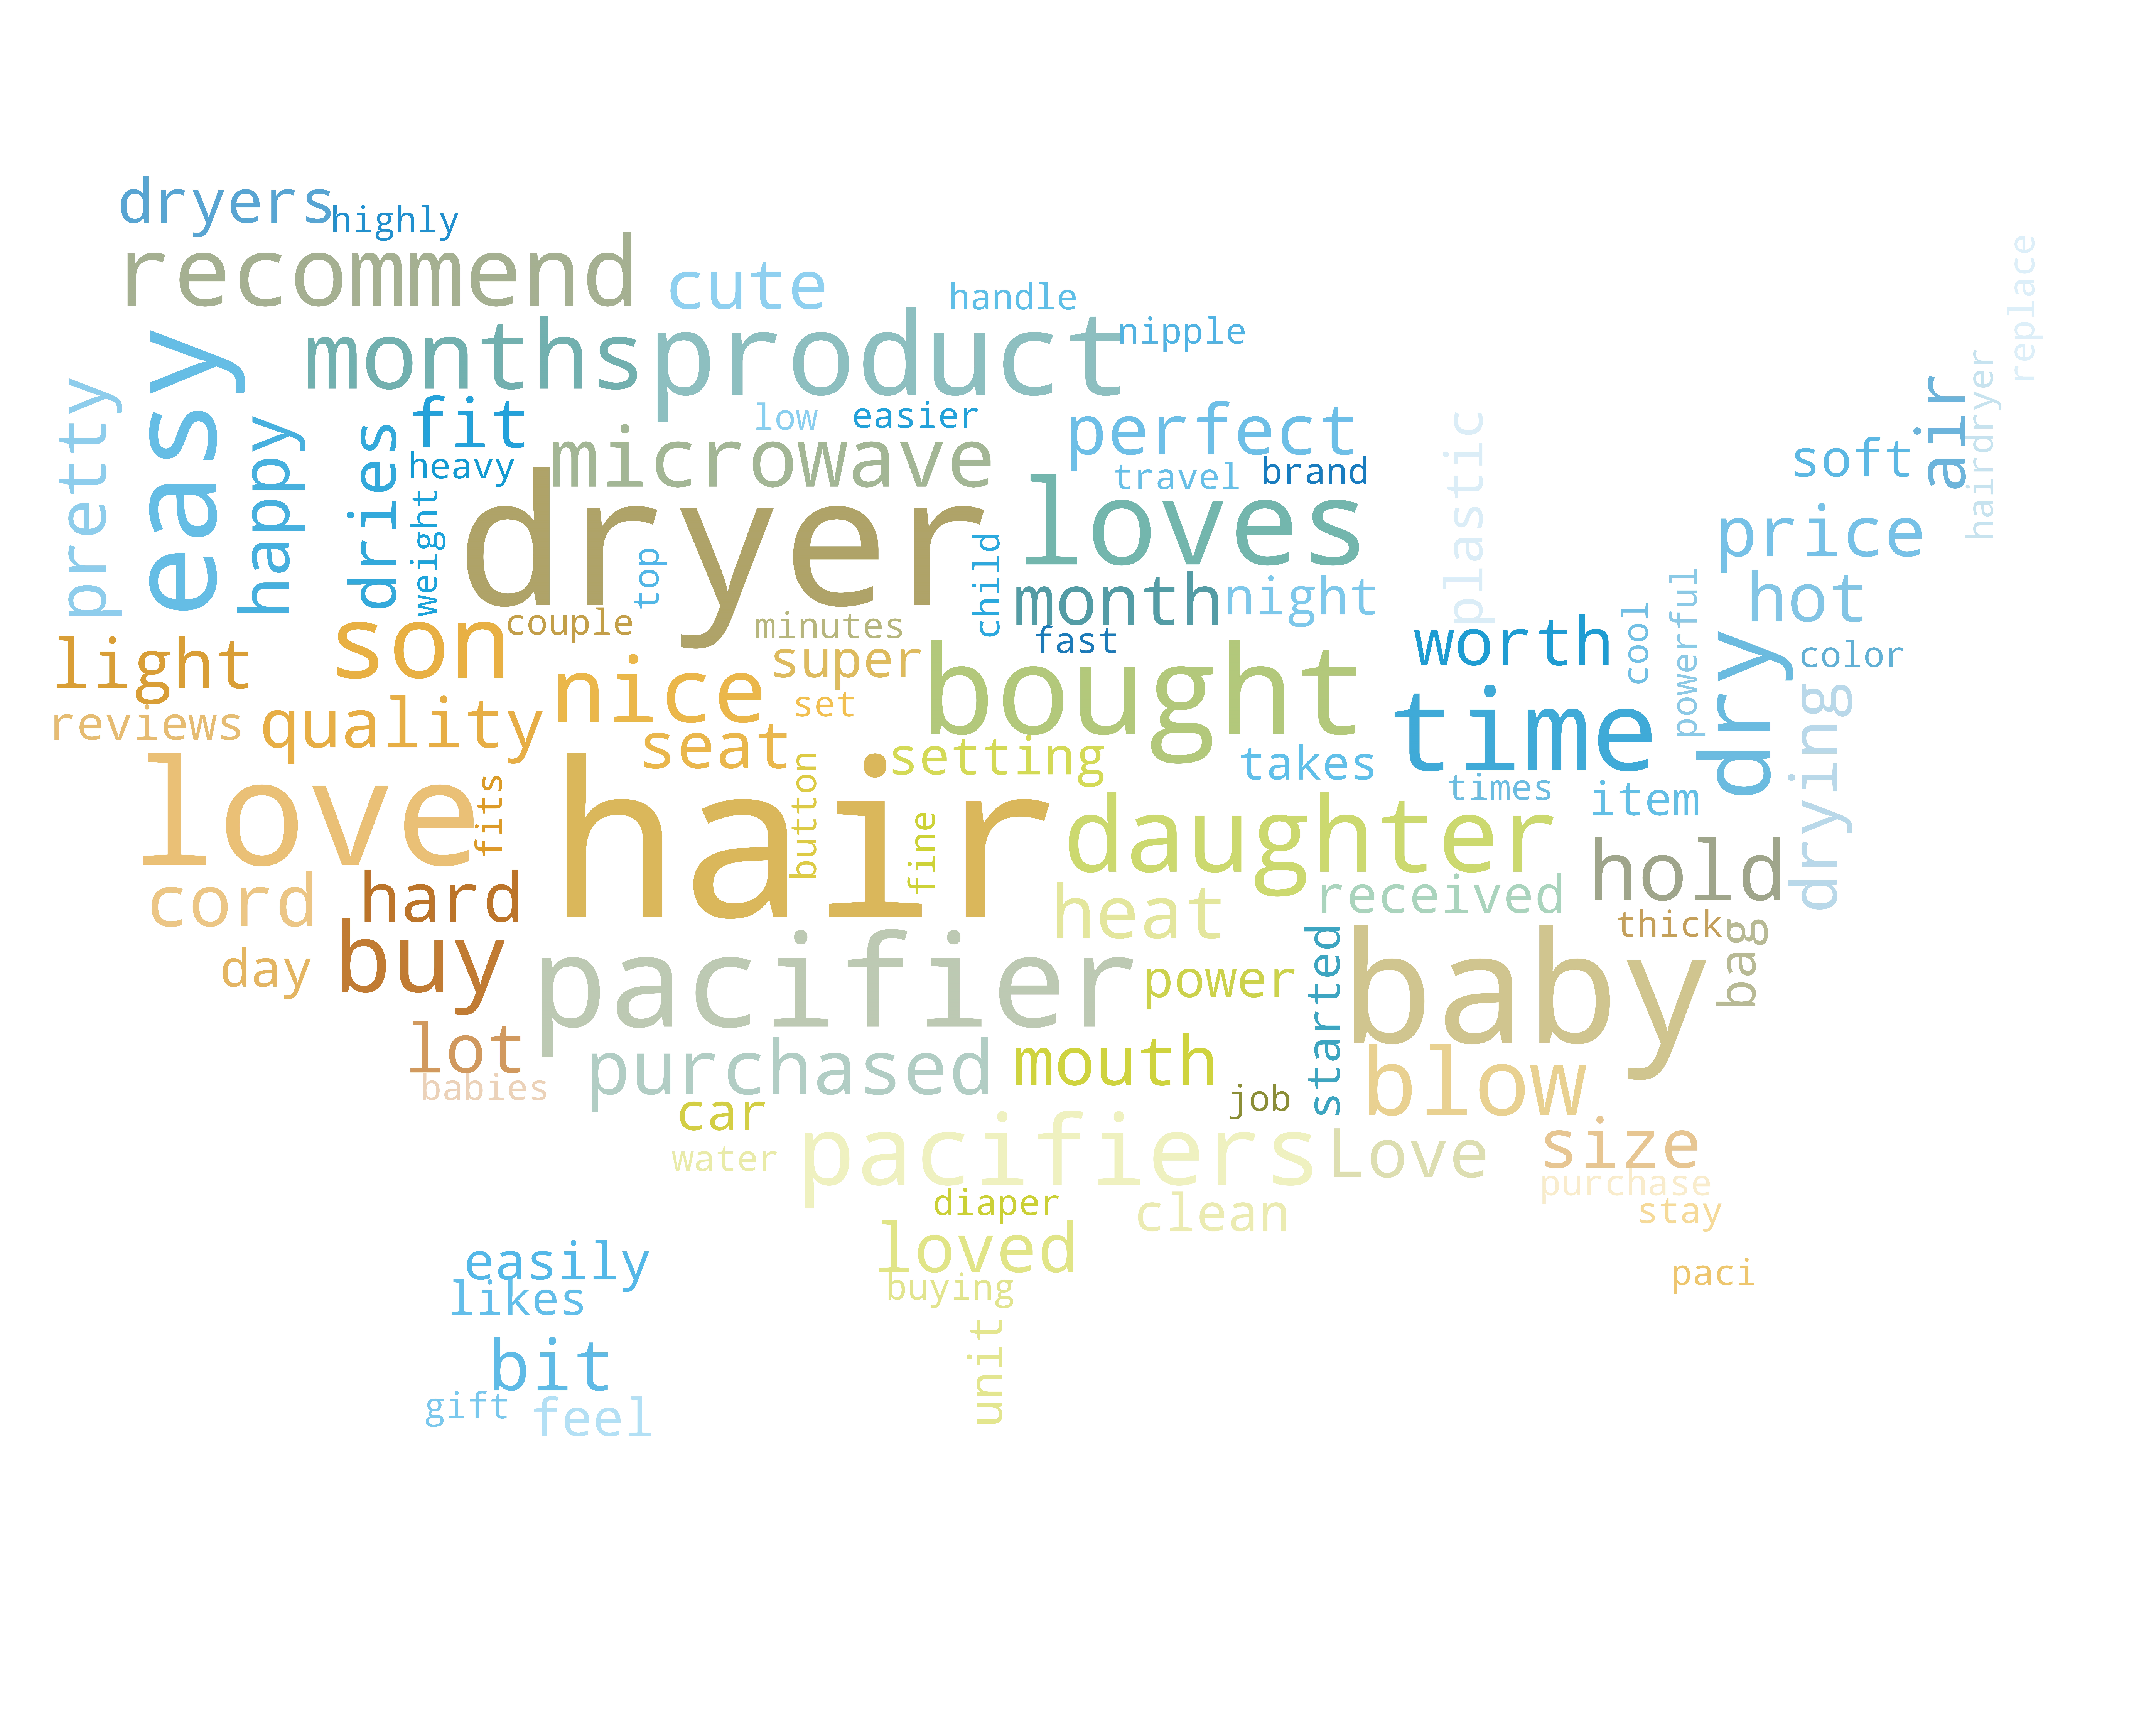
\includegraphics[width=8.5cm]{./figures/wc.png}
	\caption{The word cloud map of all comments in three data sets} \label{wordCloud}
\end{figure}
\newpage
According to the figure \ref{wordCloud}, consumers are most concerned about the quality and price of products. When products are launched on the online market, both the quality of the products and the "beautiful" price should be guaranteed.

\subsection{Potentially Important Design Features}

In the study of consumer reviews, we use the word frequency algorithm to get the high-frequency words corresponding to the stars of each product. We can find that quality, service, and price are the most important concerns for consumers. Now we want to understand the potentially important design features of specific products to enhance product satisfaction. Due to the space limitation, we will only give the frequency table of baby pacifier words.

\begin{figure}[h]
	\centering
	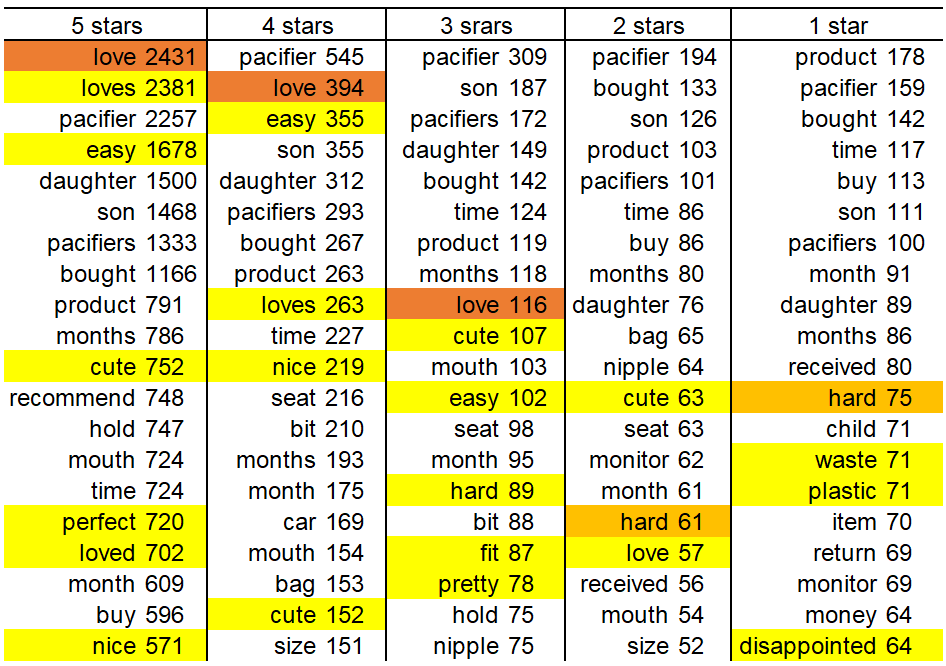
\includegraphics[width=14cm]{./figures/pdc2.png}
	\caption{Top20:The frequency of words corresponding to different stars of the baby pacifier} \label{pdc1}
\end{figure}

Bad reviews are what we're really focused on, where we can identify areas where consumers are dissatisfied,so we adjust our product or online sales strategy to improve our competitiveness. As can be seen from the figure \ref{pdc1} :

1. When evaluating products, consumers prefer to describe their subjective feelings rather than product attributes.

2. Specific quality descriptors of text-based reviews such as' love ', 'disagree', and others, strongly associated with rating levels.

3. In the low-star rating, "hard" and "plastic" reflect that the potentially important design functions of the baby nipple are its hardness and material safety; Potentially important design functions of the hairdryer are drying effect and service life. Potentially important design features of microwave ovens are functional diversity and after-sales service.

\subsection{The Product’s Reputation}

Consumers' real evaluation score only considers the content and stars of the review, not the importance of the review. The four most important factors when considering product reputation are star rating, reviews, vine, and helpful votes\upcite{WannThe}.

Each commenter contributes $p_{I}$to the product's reputation:

\begin{equation}\label{q2}
p_{i}=\sum_{i}^{n_i}[s_{i}+k_{i}(r_{i1}+r_{i2})]
\end{equation}

The reputation of a product takes into account the reputation of the product rated by each reviewer at a certain point in time, and the following indicators are obtained. This indicator can describe the reputation of the product in a certain period, whether it goes down or up, where $n_k$ is the number of reviews of j product in the k month. K month reputation score of j product $rp_{jk}$:

\begin{equation}\label{gs1}
rp_{jk}=\frac{\sum_{i}^{n_k}[s_{ji}+k_{ji}(r_{ji1}+r_{ji2})]}{n_i}
\end{equation}

In drawing the presentation, we did some manipulation on the data: each reviewer's reputation for the product was divided into $rp_{I}$by converting it to a number on $[-1,1]$. The value on $(0,1]$indicates that each reviewer's contribution to the product's reputation is positive; The value on $[-1,0)$indicates that each reviewer has a negative reputation contribution to the product; 0 indicates that each reviewer has no reputation contribution to the product; since the maximum number of baby pacifiers is 18,939, the data we selected is pacifier data.

\begin{figure}[h]
	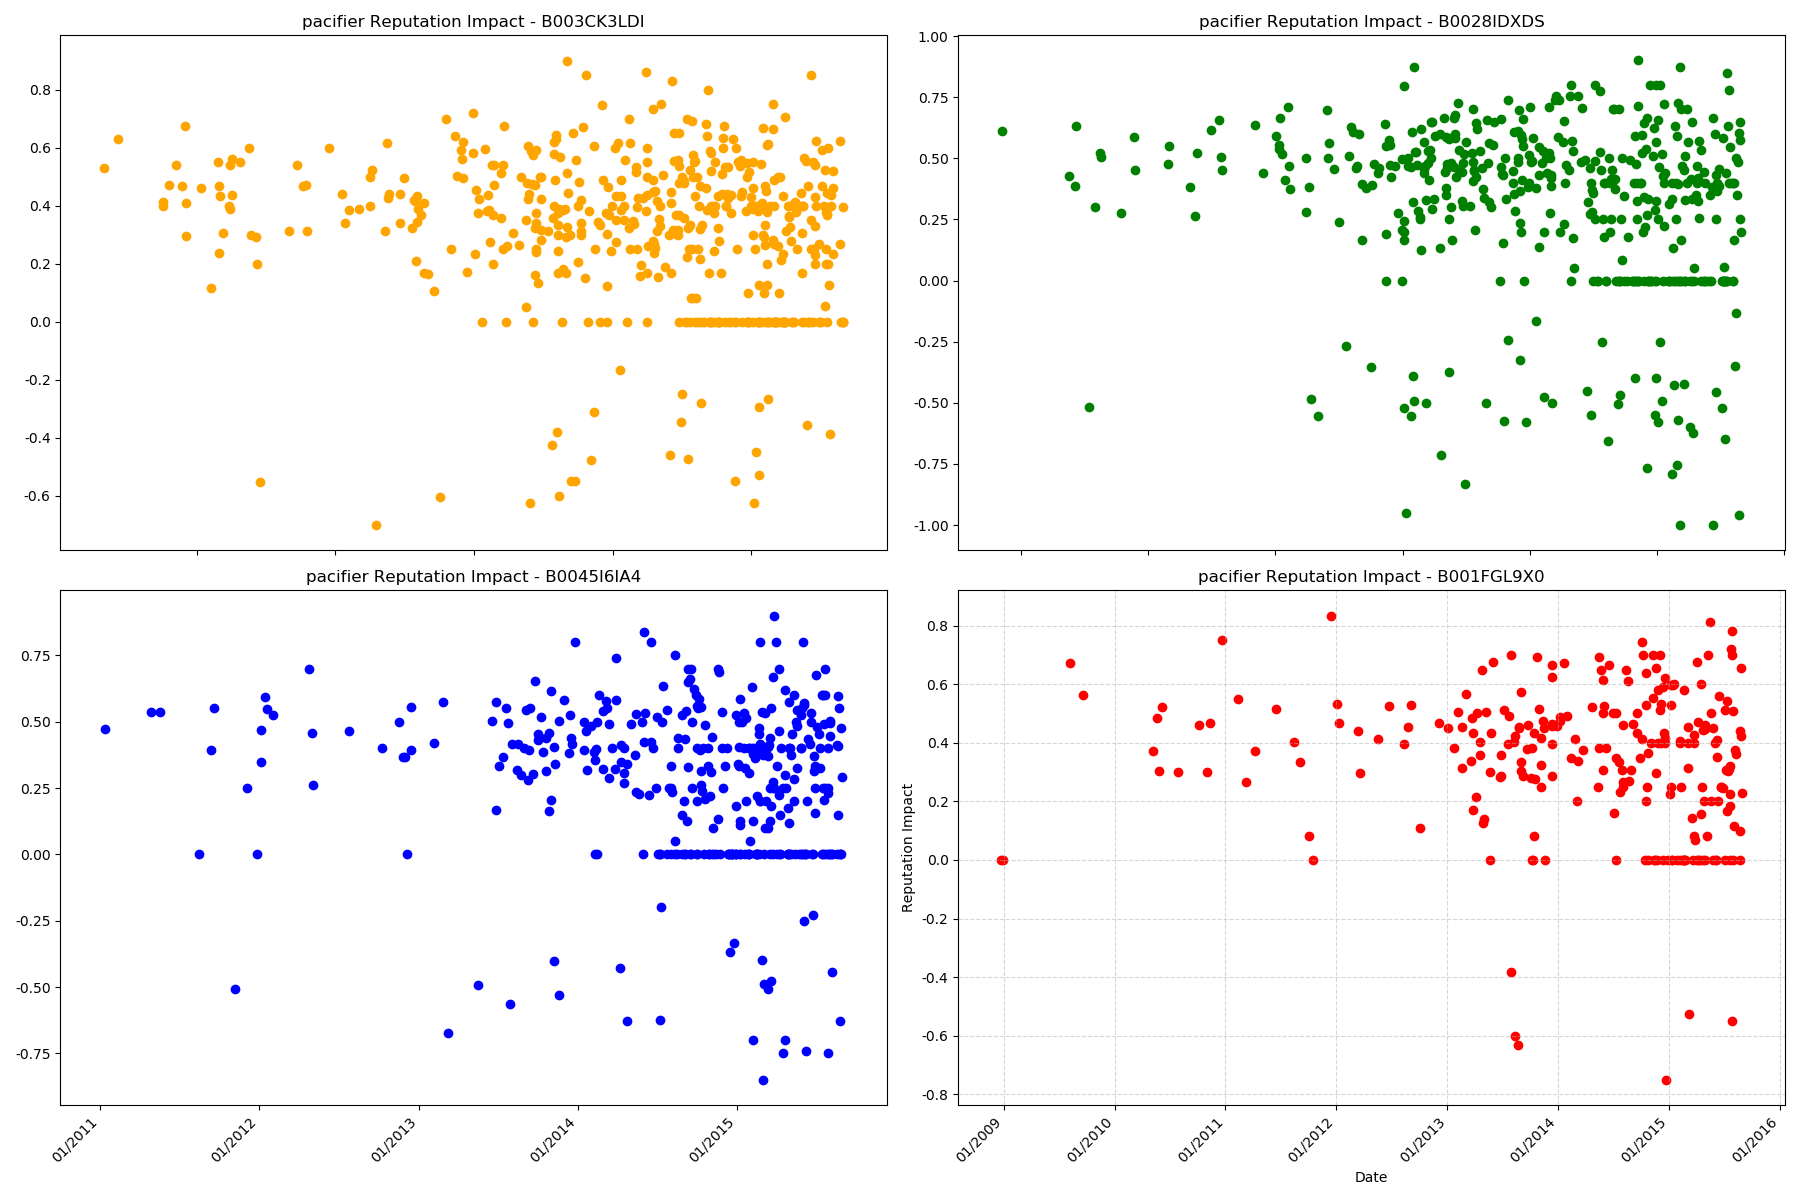
\includegraphics[width=7cm]{./figures/q2p1p.png}
	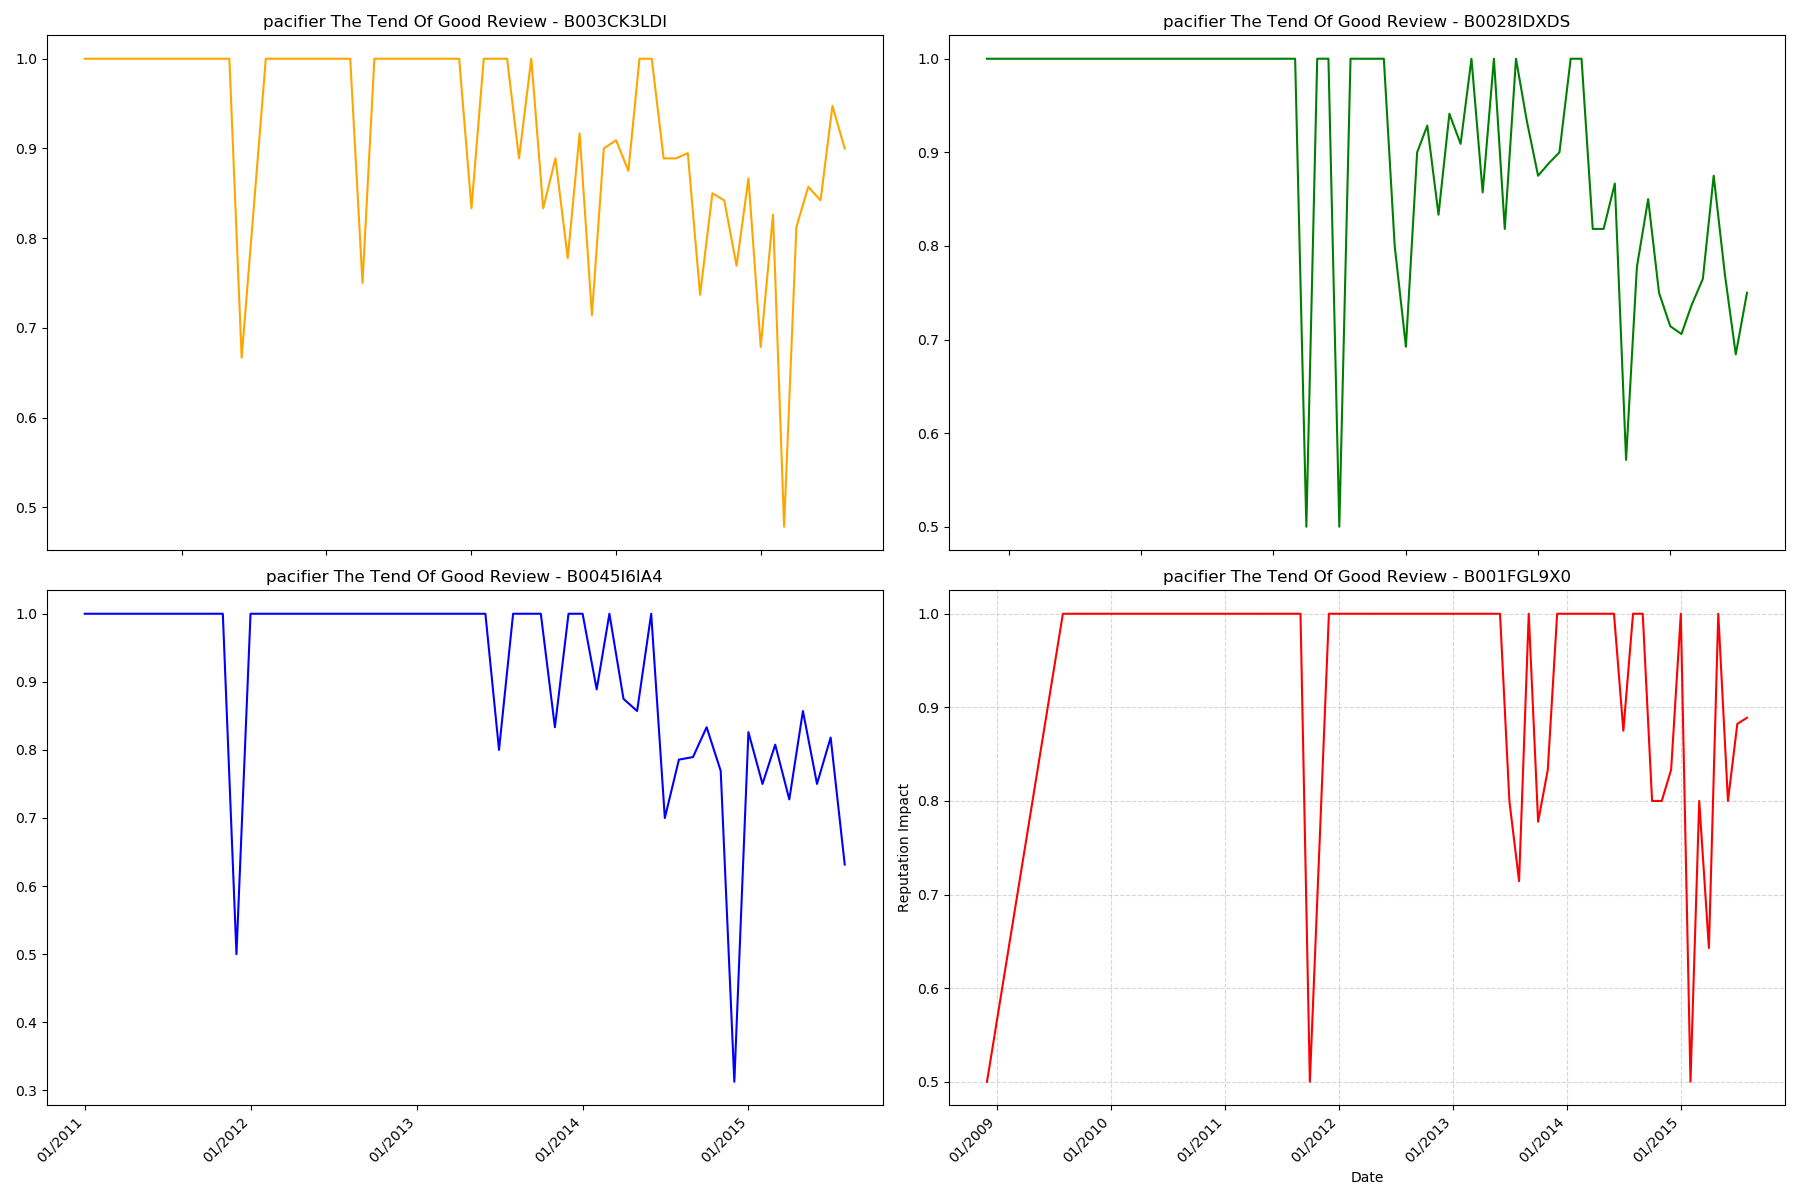
\includegraphics[width=7cm]{./figures/q2p2p.png}
	\caption{Left: reputation score of each reviewer of the top four products reviewed in the baby pacifier data; Right: monthly reputation scores for the top four products reviewed in the baby pacifier data} \label{q2p1}
\end{figure}

Figure \ref{q2p1} shows that the reputation scores of the top four products with the number of comments are mostly concentrated above 0, which indicates that most people have positive comments on the products (the same conclusion as the figure \ref{z1_q1p1} on the right). Here we are looking at the top four products in terms of the number of reviews, so these products also have high sales.

Figure \ref{q2p1} the right graph studies the proportion of the number of five-star comments to the total number of comments in a month. Reputation scores are stable at 0.5 or above, and the occasional five-star review for the month is good for the sales company. Around 2015, reputation took a turn for the worse and then stabilized. As online shopping becomes more and more common and the review data keeps increasing, it is not possible to display every comment on the shopping platform, so the network companies make corresponding adjustments to the display of comments on the shopping platform.

To sum up, sales and reputation are closely related, we strongly suggest that the sunshine company should pay attention to the reputation of products.

\subsection{The Future Trend of the Product }

How do we define success after a product has been sold in an online marketplace? If the product has been bought by many people, the comments after purchase are mostly positive, and the product has a good reputation on the Internet, then the future trend of the product must be good.

\begin{figure}[h]
	\centering
	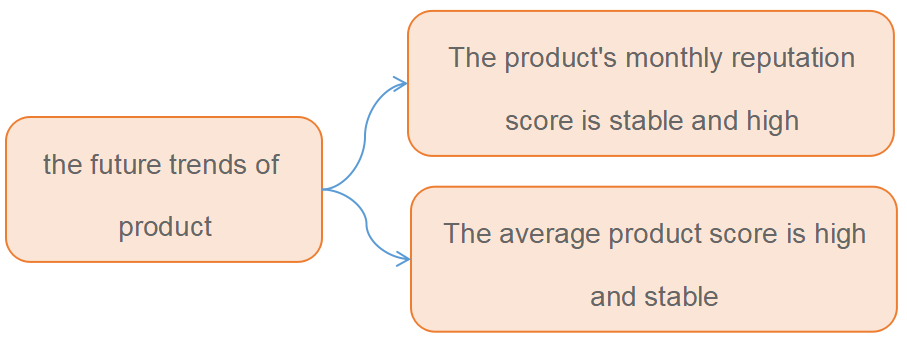
\includegraphics[width=7cm]{./figures/q3p1.png}
	\caption{the combination to indicate a potentially successful or failing product.} \label{q3p11}
\end{figure}

Reputation score and product score are important factors affecting the future development of a product. According to the formula \ref{q1}, it can be known that the product score $f3_i$is a comprehensive indicator to measure the product quality. According to the formula \ref{gs1}, we can know that the reputation score will affect the future sales of the product. These two indicators, one to measure the quality of product attributes, the other reflects the social value, together they can have a comprehensive forecast of the future trend of the product. Product future development score $\psi$:

\begin{equation}\label{gs4q1}
\psi_j=\mathbf{avg}\sum (f_{2jk}+rp_{jk})
\end{equation}

\begin{table}[h]	
	\caption{Comparison of three indicators for different products}\label{biao4q1}
	\centering
	\begin{tabular}{ccccc}
		& & & & \\
		\toprule &review number & product score  & product reputation  & total  \\
		product id &$n_j$ & $f_{2j}$ & $rp_{j}$ & $\psi_j$ \\
		\midrule B0009XH6TG & 555 & 53.76 & 13.30 & 67.06 \\
		B00VRN7SB8 & 15 & 3.37 & 16.00 & 19.37 \\
		B005GSZB9Q & 78 & 13.53 & 15.42 & 28.95 \\
		B00NXRHIO8 & 13 & 4.57 & 17.62 & 22.18 \\
		B003CK3LDI & 515 & 54.13 & 13.04 & 67.17 \\
		B00UH2XBOS & 14 & 2.65 & 13.31 & 15.96 \\
		\bottomrule
	\end{tabular}
\end{table}
\newpage
From the table \ref{biao4q1}: the more reviews the product has, the higher the future development score. Because the more reviews a product sells, the more reviews there are, the more reviews there are, so the number of reviews indirectly represents the number of sales. If we can prove that the number of comments is positively correlated with the score of future development, then it can be shown that the higher the score of $\psi_j$in future development, the more sales will be generated and the more successful the product is likely to be.

\subsection{Do specific star ratings incite more reviews?}

Question d requires an analysis of whether the customer ’s comments will be affected by the product ’s existing ratings, and emotionally biased during the review. So we will explore the impact on a certain number of previous product ratings on the sentiment of review content before user reviews.

We first calculate the average of the last 10 order ratings for each of the three categories of products, and filter out orders for less than 10 reviews, and rate the average of stars for the last 10 order ratings. Record it as Ras, and use it as the average situation reflected by a certain number of star ratings before the time node of the current order. Then explore the correlation between it and the sentiment of the comment after the time node. To simplify the condition, we use the value of Polarity to express the sentiment of the review,record it as K.

According to the above, we value the Polarity data according to the range of negative, middle and positive reviews. To make Polarity numerically correspond to ratings.We change the product score of formula \ref{m1gs1}  to
\begin{equation}\label{q5gs1}
K=1.5K_i
\end{equation}

\subsubsection*{Canonical correlation analysis}

In 1936, Hulling proposed canonical correlation analysis to reveal the linear correlation between two groups of multivariate random variables. In order to further to extract the correlation between the two sets of variables, Ras and K, we decided to use canonical correlation analysis, which uses the idea of principal component analysis to find the linear combination of input variables and output variables, and then discuss the linear combination Related relationship. \upcite{jj}

We first assume that these two sets of data follow a joint normal distribution.

Assuming\(\mathbf{X}=\left[\begin{array}{l}
\mathbf{X}^{(1)} \\
\mathbf{X}^{(2)}
\end{array}\right]\) follows a normal distribution \(N_{p+q}(\boldsymbol{\mu}, \boldsymbol{\Sigma})\),Select a sample of sample size n from the population to obtain the following data matrix:

\[\mathbf{X}^{(1)}=\left[\begin{array}{cccc}
X_{11}^{(1)} & X_{12}^{(1)} & \cdots & X_{1 p}^{(1)} \\
X_{21}^{(1)} & X_{22}^{(1)} & \cdots & X_{2 p}^{(1)} \\
\vdots & \vdots & \ddots & \vdots \\
X_{n 1}^{(1)} & X_{n 2}^{(1)} & \cdots & X_{n p}^{(1)}
\end{array}\right]\]

If the overall canonical correlation coefficient is \(\lambda_{k}=0\),then there is no correlation between the corresponding canonical variables \(U_{k}\) and \(V_{k}\).Therefore, it has no effect on the analysis of the impact of \(X^{(1)}\) on \(X^{(2)}\). Such typical variables can be disregarded, so how to determine whether the overall typical correlation coefficient is zero according to the sample data, in order to determine the problem that several typical variables should be taken.

Bartlett proposed a hypothesis testing method. The test method is to check whether the overall typical correlation coefficient \(\lambda_{1}, \lambda_{2}, \cdots, \lambda_{r}\) is equal to zero based on the sample data.

Hypothesis tests is:

\[\begin{aligned}
&H_{0}: \lambda_{k+1}=\lambda_{k+2}=\cdots=\lambda_{r}=0\\
&H_{1}: \lambda_{k+1} \neq 0
\end{aligned}\]

In order to study the correlation between the two indicators of RAS and \(K_{i}\), we let RAS be the input variable and \(K_{i}\) be the output variable. The results obtained by SPSS software are as follows:

\begin{table}[h]
	\centering
\caption{Set1 $\&$ Set2 Standardized Canonical Correlation Coefficients}\label{q4b1}

	\begin{tabular}{cccc}
		& & & \\
		\toprule Set1 Variable &  & Set2 Variable &  \\
		\midrule H polarity & $-0.073$ & H star average & $-0.257$ \\
		P polarity & $-0.991$ & P star average & $-0.946$ \\
		M polarity & $-0.137$ & M star average & $-0.273$ \\
		\bottomrule
	\end{tabular}
	
\end{table}



Then according to Table \ref{q4b1}, the first pair of Standardized Canonical Correlation Coefficients can be obtained as follows:

\[\begin{aligned}
&U_{1}^{*}=-0.073 Z_{1}^{(1)}-0.991 Z_{2}^{(1)}-0.137 Z_{3}^{(1)}\\
&V_{1}^{*}=-0.257 Z_{1}^{(2)}-0.946 Z_{2}^{(2)}-0.273 Z_{3}^{(2)}
\end{aligned}\]

Where in, \(Z_{i}^{(1)}\)and\(Z_{j}^{(2)}\) are the result of the original standardized variables \(X_{i}\) and \(Y_{j}\).

The above results show that P polarity, which is the sentiment score of Pacifier's text content, is -0.991 in the first group of typical related variables. The larger the absolute value of the data, the greater the importance. P stars average indicators, it is Ras of Pacifier. Its importance of the first group of canonical correlation variables is -0.946. Similarly, we can also get the importance of the other two variables in the two sets in the first canonical correlation variable.

\begin{table}[h]
	\centering
	\caption{Canonical Correlations}\label{q4b2}
	\begin{tabular}{ccccccc}
		& & & \\
		\toprule  Correlation & Eigenvalue & Wilks  & $\mathrm{F}$ & $\mathrm{Num} $ & Denom  & Sig. \\
		&  &  Statistic &  & D.F. &  D.F. &  \\
		\midrule  0.14 & 0.02 & 0.972 & 2.14 & 9.00 & 1625.89 & 0.024 \\
		0.09 & 0.01 & 0.992 & 1.34 & 4.00 & 1338.00 & 0.254 \\
		0.02 & 0.00 & 0.999 & 0.36 & 1.00 & 670.00 & 0.552 \\
	\bottomrule
	\end{tabular}
\end{table}

From Table \ref{q4b2}, it can be seen that the value of the Significance analysis in the Canonical Correlations of the first pair of typical variables is 0.024. In the case of \(\alpha\) = 0.05, 0.024 <0.05, indicating that the null hypothesis is rejected at a \(95 \%\) probability, that is The correlation to typical variables is significant, indicating a strong correlation to RAS and K indicators. Significance analysis values of the typical correlation coefficients of the second and third pairs of typical variables are 0.254 and 0.552, respectively, so the correlation between the second and third pairs of typical variables is not significant when \(\alpha\) = 0.10. It shows that there is only one pair of typical variables between the two indicators of RAS and K.

In general, through analysis of typical related variables, it can be concluded that the content of customer reviews will be affected by the star rating of previous order reviews.

\subsection{ Is the comment content  related to the rating level?}

Before exploring the relevance to review content and ratings, we first perform descriptive statistics on several quantitative data onto all sample data in order to have a general understanding of the characteristics of the data.

\begin{table}[h]	
	\caption{Descriptive statistics for reviews and ratings and votes}\label{biao5q1}
	\centering
	\begin{tabular}{ccccccc}
		& & & & & & \\
		\toprule &&\text { Star Rating } & && \text { Polarity } \\
		& \text {H  } & \text { M } & \text {P  } & \text {H  } & \text {M  } & \text {P  } \\
		\midrule \text { Mean } & 4.116 & 3.445 & 4.305 & 0.264 & 0.215 & 0.282 \\
		\text { Standard error} & 0.012 & 0.041 & 0.009 & 0.003 & 0.0068 & 0.002 \\
		\text { Minimum } & 1.000 & 1.000 & 1.000 & -1.000 & -1.000 & -1.000 \\
		\text { Maximum } & 5.000 & 5.000 & 5.000 & 1.000 & 1.000 & 1.000 \\
		\bottomrule
	\end{tabular}
\end{table}

As can be seen from Table \ref{biao5q1}, in terms of product ratings, the average rating of Pacifier is the highest among the three products, and the average rating of Microwave is the lowest. In terms of review types, judging from their averages, consumers who buy Pacifier have higher averages of extreme content, and they are more inclined to praise such products. Consumers who buy Microwave have the lowest averages. This reflects the positive correlation between the rating and the type of content evaluated to a certain extent. At the same time, the standard deviation of Pacifier product ratings and review types are the smallest among the three types of products, indicating that most of the values of the two types of data have small differences between their average values and the data is relatively stable. There is no significant difference between the maximum and minimum product ratings and product reviews for the three types of products.

Then let ’s explore the relevance to review content and ratings.

As can be seen from Figure \ref{q5p1}, in the percentage histogram of Pacifier product data, as the rating increases, the proportion of positive reviews in total numbers of reviews gradually increase, and the number of negative reviews in the total number of reviews The proportion gradually decreases. It can be seen that there is a certain correlation between the rating and the content of the review. A high probability of a customer with a high rating order also gives a positive comment, and a review of a low rating order is more likely to have a bad review. And the proportion of the middle rating in the five ratings is the lowest, indicating that consumers are more inclined to give extreme reviews, and extreme praise is the majority. The other two categories of products also meet this feature.

\begin{figure}[h]
	\centering
	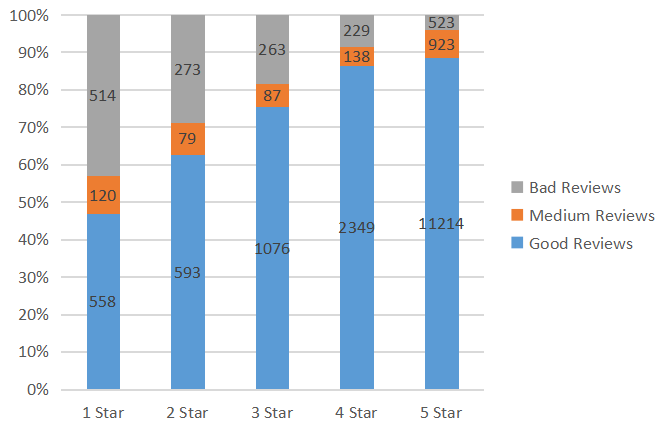
\includegraphics[width=8cm]{./figures/q5p1.png}
	\caption{Pacifier product rating and review type percentage histogram} \label{q5p1}
\end{figure}

The model in this section is mainly to study the correlation between the two sets of variables of the extreme value of the review and the rating. In Excel, we calculated the Polarity data we obtained using TextBlog. We have counted the number of three review types of three categories of products of different ratings. Calculate the Pearson correlation coefficient of the data, and hope to get the correlation between the type of review and the rating. The formula for calculating the Pearson correlation coefficient is as follows:
\begin{equation}\rho_{X Y}=\frac{\operatorname{Cov}(X, Y)}{\sigma_{X} \sigma_{Y}}=\frac{\sum_{i=1}^{n} \frac{\left(X_{i}-E(X)\right)}{\sigma_{X}} \frac{\left(Y_{i}-E(Y)\right)}{\sigma_{Y}}}{n}
\end{equation}

Use the sample data to calculate the value of $\rho_{X Y}$, which ranges from -1 to 1. $\rho_{X Y}$> 0 indicates that there is a positive correlation between the two variables, otherwise it is a negative correlation; $\rho_{X Y}$ = 0 indicates that there is no correlation between the variables; |$\rho_{XY}$|> 0.8 indicates a strong correlation between the variables, 0.3 indicates that the correlation between variables is very weak and can be considered irrelevant \upcite{ww}.

\begin{figure}[h]
	\centering
	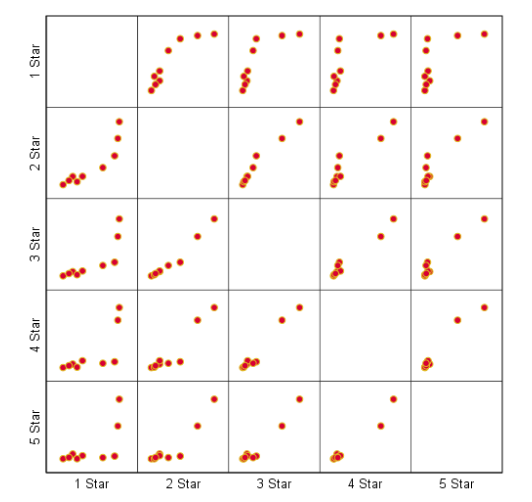
\includegraphics[width=7cm]{./figures/q5p2.png}
	\caption{Matrix scatter plot of Star Ratings} \label{q5p2}
\end{figure}

The data onto each star is composed of three types of data onto positive and negative reviews. According to Figure \ref{q5p2}, it can be seen that the data onto different stars has a strong positive correlation. Then we explore the correlation between the type of text review and Star Rating by calculating the Pearson correlation coefficient.

\begin{table}[h]
	\caption{Correlation results}\label{q5b1}
	\centering
	\begin{threeparttable}
		\begin{tabular}{cccccc}
			& & & & & \\
			\toprule & 1 star & 2 star & 3 star & 4 star & 5star \\
			\midrule 1star & 1.00000 & $0.89767^{* *}$ & $0.81339^{* *}$ & $0.73236^{*}$ & $0.66760^{*}$ \\
			2star & $0.89767^{* *}$ & 1.00000 & $0.98154^{* *}$ & $0.94018^{* *}$ & $0.92027^{* *}$ \\
			3star & $0.81339^{* *}$ & $0.98154^{* *}$ & 1.00000 & $0.98349^{* *}$ & $0.97387^{* *}$ \\
			4star & $0.73236^{*}$ & $0.94018^{* *}$ & $0.98349^{* *}$ & 1.00000 & $0.97954^{* *}$ \\
			5star & $0.66760^{*}$ & $0.92027^{* *}$ & $0.97387^{* *}$ & $0.97954^{* *}$ & 1.00000 \\
			\bottomrule								
		\end{tabular}
		\begin{tablenotes}
			\footnotesize
			\item[1] \(* *.\)Correlation is significant at the 0.01 level (2-tailed). 
			\item[2] \(*.\)Correlation is significant at the 0.05 level (2-tailed).
		\end{tablenotes}
	\end{threeparttable}
\end{table}

It can be seen from Table \ref{q5b1} that the correlations between the variables are relatively large, and the absolute values are all above 0.65. It can be considered that there is a strong positive correlation between the variables. Only the data onto Star Rating of 1 and the data onto Star Rating of 4 and 5 are relatively weak, which is significant at the \(95 \%\) level. The correlations between the other Star Rating variables were stronger, significant at the \(99 \%\) level. In addition, it can be seen that the correlation between the data with a Star Rating of 1 star and other data, as the star rating of the Star Rating data increases, the correlation between the data with a Star Rating of 1 star and other data gradually decreases. The data onto a Star Rating of 5 stars has a similar relationship. The correlation between it and other data increases to the Star Rating data stars starting from 1 star, and the correlation between the Star Rating data onto 5 stars and other data gradually increases.

This first illustrates the different ratings consumers give to products, and the correlation between the three types of data onto their evaluation content is relatively strong. Orders for a rating of 1 star and a rating of 5 stars have a lower correlation between their review content types.
%\begin{comment}
\section{Model Improvement}

In the selection of stop words, specific quality descriptors of comments such as "good", "great" will not be used as stop words, and the word frequency and frequency will be obtained. We will update the graph \ ref {wordCloud} and the graph \ ref {pdc1}. In the display of the problem-solving ideas, you can choose the frequency of words with different parts of speech corresponding to different stars, and understand the frequency of appearance of verbs, adjectives, and nouns, which will be more conducive to our analysis of product conditions.

When discussing the future trend of the product, we got points for the future development of the product. In this article, only part of the data is displayed. A linear model of the number of reviews and the future development score of the product should be established, and the correlation should be tested to find the correspondence between the number of reviews and the number of reviews and the future development score of the product. 

\section{Sensitivity Analysis}

In this article, the weights of star ratings reviews effective scores, and evaluation scores in consumer real evaluation scores and product scores are fixed values. But we know the weight and reality of the two target activities (sales strategy and product design features) we face because different consumer impacts can be differently
related. Therefore, we calculated 10 sets of results for $0.1,0.2, \cdots, i$ to test the sensitivity and feasibility of the model. In the actual consumer evaluation score, there is a big jump between $\phi = 0.4$ and $\phi = 0.6$; the product score is between $\ phi = 0.2$ and $\phi = 0.4$. When the values of the parameters are close to these thresholds, the calculation results are hardly affected. However, when the value is far from the threshold, the sensitivity is very high. Therefore, $\phi$ and $\eta$ should be based on the actual situation, especially when the value is close to the threshold.


\section{Strengths and Weaknesses}

\textbf{Strengths}
	\begin{itemize}
		\item More comprehensive and objective indicators
		
			When looking for and selecting indicators for a product, we consider its equations as thoroughly and as carefully as possible. It is associated with most of the indicators in the data set, which means that our model is a valid and meaningful basis.
		
		\item The model compares the correct results
		
		With a limited number of indicators and data, the results of the model are still more in line with objective facts. In particular, the results highlight the impact of product metrics, product reputation, and other metrics on product success, which are novel and effective.
		
		\item Extensive measurement mode
		
		In our model, we select metrics based on three aspects: star rating, help rating, and review content. We design metrics that reflect product scores, product reputation, and product potential.
		
		\item Intuitive results
		
			In different models, we have used a large number of charts to show our analysis and results, and have adopted novel ways to display, such as word cloud diagrams, which can more intuitively understand the trend of product-related parameter changes.
		
		\item Good scalability
			The data mining and analysis of the data set and the drawing of the time series diagram are all completed by Python code, which has extremely high scalability. For example, in terms of stopword selection, we can modify it according to our actual situation, including waiting for stopwords and keywords, so that the results will be more accurate.
		
	\end{itemize}
	
	
\textbf{Weaknesses}
	\begin{itemize}
	
	\item Subjectivity and limitations in the process of indicator selection.
	
	Although reference is made to relevant literature and influencing factors of objective facts, a subjective overview is still selected
	Read indicators. But without enough literature and comprehensive data, this is inevitable.
	
	\item Errors caused by discontinuities in time.
	
	Because the time of the data is not continuous, the measurement of time is only an approximate range
	
	\item Limitations of data
	
	In the analysis of the data, we only evaluated the conditions in the data set, and the dates were rather limited. In this way, our analysis results are not comprehensive and accurate enough to represent the sales strategy of all products online. Because historical data sets are used, this model may not be applicable if new changes or booms in online sales occur in the future.
	
	\end{itemize}
%\end{comment}
\newpage
%\thispagestyle{empty}
%\addcontentsline{toc}{section}{Reference}
%\nocite{Bibtexkey}
\bibliographystyle{plain}
\bibliography{myreference}

\end{document}


